\chapter{Lo standard IEEE 802.21}

\begin{figure}[h!]
\centering
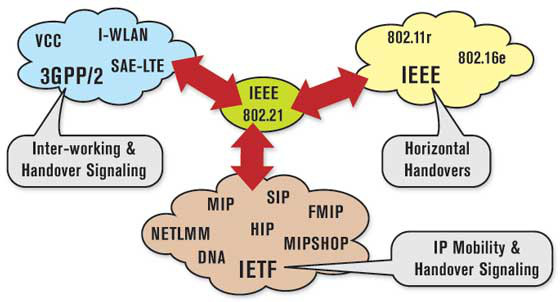
\includegraphics[scale=0.6]{ieee80221_cloud.jpg}
\caption{Rapporto con gli altri standards}
\end{figure}

In questo capitolo sarà esposto lo standard IEEE 802.21\cite{standard}, illustrandone le componenti e le loro funzionalità, al fine di avere un quadro completo e poter comprendere il suo reale obbiettivo, ovvero creare un meccanismo standardizzato per poter prendere più facilmente decisioni di {\em handover}, in modo che sia {\em media-independent}, ovvero indipendente dal mezzo trasmissivo utilizzato.

\section{Storia}
Con il continuo diffondersi di nuove tecnologie e dispositivi dotati di più interfacce di rete, è diventato necessario dover formalizzare alcune funzionalità per facilitare un passaggio indolore da una rete all'altra.
Il {\em working group} cominciò effettivamente i lavori nel marzo 2004 e la prima versione ufficiale dello standard fu pubblicata nel gennaio 2009. Gli eventi principali sono stati i seguenti:
\begin{itemize}
\item marzo 2003: creazione IEEE 802.21 ECSG\footnote{Executive Committee Study Group}
\item marzo 2004: creazione IEEE 802.21 WG\footnote{Working Group}
\item settembre 2004: analisi dei requisiti
\item ottobre 2004: raccolta delle proposte
\item maggio 2005: formulazione di una proposta unica
\item luglio 2005: inizio discussione della proposta
\item luglio 2007: IEEE 802 Sponsor Ballot\cite{balloting}
\item gennaio 2009: pubblicazione dello standard
\end{itemize}

\begin{figure}[h!]
\centering
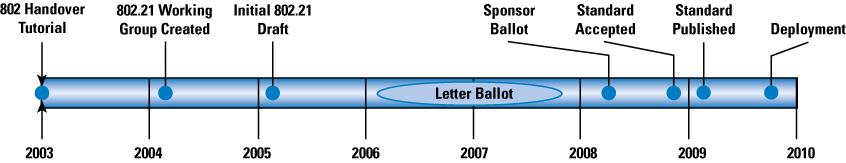
\includegraphics[scale=0.48]{ieee_timeline.jpg}
\caption{IEEE 802.21 Timeline}
\end{figure}

\section{Finalità}
Lo standard IEEE 802.21 si pone l'obbiettivo di aiutare i nodi mobili a prepararsi ad eventuali azioni di {\em handover} da una rete ad un'altra, ma non specifica come deve avvenire la migrazione. Sono infatti definite tutte le funzionalità per acquisire informazioni sullo stato delle varie interfacce, ma non è specificato come e quando debba effettivamente avvenire l'eventuale passaggio. L'utente è in grado di conoscere lo stato delle connessioni disponibili attraverso la ricezione di eventi dal proprio MIHF\footnote{Media Independent Handover Function}, quali {\em link\_up} e {\em link\_down}, e può richiedere esplicitamente informazioni aggiuntive su una interfaccia inviando delle specifiche richieste ad un particolare SAP\footnote{Service Access Point}, come l'RSSI\footnote{Received Signal Strength Indication} di una propria interfaccia 802.11 attualmente connessa. Lo standard 802.21 da solo non basta per gestire i meccanismi di {\em handovers}, poiché, ad esempio, per riuscire ad effettuare una migrazione {\em seamlessly} delle connessioni attualmente attive, mantenendo quindi lo stato dei flussi aperti prima e dopo l'{\em handover}, sarebbe necessaria anche una migrazione dell'indirizzo di terzo livello attraverso, ad esempio, Mobile IP\cite{mobileip}, altrimenti, anche dopo aver instaurato con successo la nuova connessione, il {\em peer} remoto non potrebbe sapere il nuovo indirizzo del nodo a cui era connesso precedentemente.

\section{Architettura}
Lo standard IEEE 802.21 definisce più entità, ognuna con il proprio specifico compito:
\begin{itemize}
\item MIHF: implementa il core delle funzionalità offerte dallo standard.
\item MIH-SAP: fornisce una astrazione {\em media-independent} per tutti i tipi di interfacce.
\item MIH-LINK-SAP: fornisce una astrazione {\em media-specific} per una singola tecnologia.
\item MIH-NET-SAP: permette la gestione di MIHF remoti.
\item MIH-User: è l'entità che si sottoscrive ad un MIHF per usufruire dei servizi offerti.
\end{itemize}

\begin{figure}[h!]
\centering
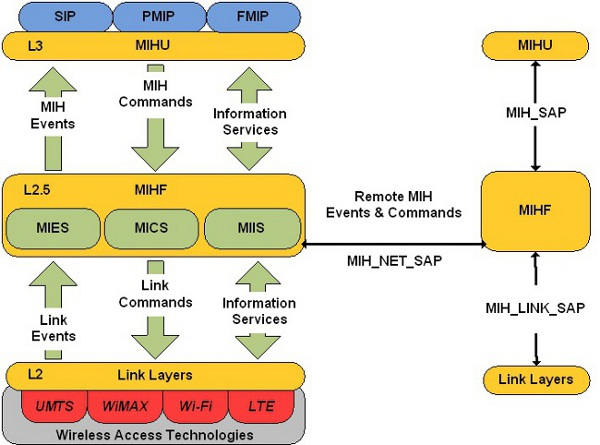
\includegraphics[scale=0.9]{ieee80221.jpg}
\caption{Architettura IEEE 802.21}
\end{figure}
\subsection{MIHF}
Questo componente è il più importante: i nodi mobili devono sottoscriversi ad un MIHF, il quale invierà loro una conferma con informazioni sui collegamenti disponibili, come i rispettivi indirizzi di livello due ed il tipo di tecnologia, ed un elenco di eventi e comandi supportati. In sostanza, l'MIHF fornisce un insieme di servizi astratti ai livelli superiori indipendentemente dalle tecnologie adottate dalle singole interfacce.
L'implementazione della Media Independent Handover Function è formata da tre sottocomponenti:

\begin{itemize}
\item MIES (Media Independent Event Services): ha il compito di propagare gli eventi a tutte le parti interessate come cambiamenti dinamici dello stato a livello {\em data link}, i.e. il secondo strato dello stack di rete, agli strati soprastanti del sistema locale o di sistemi remoti. Gli eventi possono essere generati dall'MIHF stesso oppure dai livelli sottostanti. Il flusso dei dati generati da questo componente ha quindi un verso prettamente {\em bottom-up}.

\begin{table}[h]
\begin{tabular}{|p{0.35\textwidth}|p{0.65\textwidth}|}
\hline
Nome & Descrizione \\
\hline
\hline
Link\_Up & il collegamento L2 torna attivo \\
\hline
Link\_Down & il collegamento L2 cade  \\
\hline
Link\_Detected & nuovo collegamento disponibile \\
\hline
Link\_Going\_Down & il collegamento sta per saltare \\
\hline
Link\_Handover\_Imminent & sta per essere eseguita una procedura di {\em handover} \\
\hline
Link\_Handover\_Complete & la procedura di {\em handover} è stata completata \\
\hline
\end{tabular}
\caption{Lista degli eventi specificati nello standard}
\label{mihevents}
\end{table}

\item MICS (Media Independent Command Services): è incaricato di propagare i comandi ricevuti dagli strati più alti dello stack di rete verso il basso per aiutare il nodo mobile ad eseguire più facilmente procedure di {\em handover}, ad esempio una richiesta esplicita per la riconfigurazione per un'interfaccia, per comunicare ad un MIHF remoto di procedere con l'esecuzione di un {\em handover} oppure una richiesta di informazioni più dettagliate sullo stato di un collegamento specifico, e.g. richiedere il valore RSSI di un'interfaccia wireless. I comandi possono essere originati sia dall'MIH-User, sia dall'MIHF stesso. La destinazione dei comandi può essere per i livelli inferiori dello stack locale oppure di uno stack remoto, propagando il comando al peer MIHF appropriato. Il flusso dei dati è prettamente {\em top-down}.

\item MIIS (Media Independent Information Services): è la componente incaricata di gestire richieste di informazioni e le opportune risposte. Ad esempio, un nodo mobile può essere interessato ad informazioni aggiuntive riguardo uno specifico link, come l'RSSI di una interfaccia 802.11, inviando una richiesta all'MIHF a cui è sottoscritto tramite il MICS ed aspettando una risposta dall'MIIS. Lo scambio di informazioni è effettuato secondo un modello RDF\footnote{https://en.wikipedia.org/wiki/Resource\_Description\_Framework} basato su XML\footnote{https://en.wikipedia.org/wiki/Extensible\_Markup\_Language}, variants\footnote{https://en.wikipedia.org/wiki/Variant\_type} oppure TLV\footnote{https://en.wikipedia.org/wiki/Type-length-value}. In questo caso non è possibile stabilire un verso per il flusso delle informazioni, poiché uno strato superiore dello stack potrebbe richiedere informazioni circa un {\em layer} sottostante o viceversa.
\end{itemize}

\subsection{SAPs}
Questo componente è incaricato di interagire con le interfacce di rete, al fine di esporre delle primitive di servizi di basso livello di una singola interfaccia ad un MIHF, al quale deve essersi preventivamente registrato.
I Service Access Points possono essere di due tipi: {\em media-independent} e {\em media-specific}.
I primi forniscono servizi astratti per tutte le possibili tipologie di interfacce di rete, come la generazione di eventi {\em link\_down} e {\em link\_up}, e, di conseguenza, offrono un minor numero di servizi.
I secondi forniscono servizi specifici per una singola tecnologia, e.g. 802.3 o 802.11, e per questo motivo sono più espressivi dei primi: ad esempio, in seguito ad una richiesta {\em get\_link\_parameter} è naturale aspettarsi risposte differenti per ogni famiglia di tecnologie, come l'RSSI che assume valori differenti a seconda della tipologia dell'interfaccia interrogata. 

\begin{table}[h]
\begin{tabular}{|p{0.37\textwidth}|p{0.63\textwidth}|}
\hline
Nome & Descrizione \\
\hline
\hline
Link\_Get\_Parameters & permette di richiedere informazioni aggiuntive riguardo un collegamento specifico \\
\hline
Link\_Configure\_Thresholds & permette di definire dei valori-soglia che facciano scattare degli eventi  \\
\hline
Link\_Capability\_Discover & permettere di ottenere la lista di eventi e comandi supportati da un MIHF  \\
\hline
Link\_Event\_Subscribe & permettere di registrarsi per essere avvisati di cambiamenti di stato di una particolare interfaccia\\
\hline
Link\_Event\_Unsubscribe & permettere di la sottoscrizione effettuata con il comando precedente\\
\hline
Link\_Actions & permette di comandare esplicitamente l'interfaccia (e.g. {\em power\_up}, {\em power\_down}) \\
\hline
Net\_Ho\_Candidate\_Query & in {\em handovers} iniziati dalla rete, segnala al nodo mobile di procedere al passaggio ad uno dei network candidati \\
\hline
Net\_Ho\_Commit & conferma all'esecuzione dell'{\em handover} \\
\hline
N2n\_Ho\_Query\_Resources & prima di confermare l'esecuzione dell'{\em handover} su un altro network, l'attuale PoS\footnote{Point of Service} contatta il candidato per controllare che abbia le risorse per accettare un nuovo nodo mobile \\
\hline
N2n\_Ho\_Commit & il passaggio verso il nuovo PoS è confermato\\
\hline
N2n\_Ho\_Complete & la procedura di {\em handover} è stata completata \\
\hline
Mn\_Ho\_Candidate\_Query & in {\em handovers} iniziati dal nodo mobile, serve per richiedere la lista dei network candidati per un eventuale passaggio \\
\hline
Mn\_Ho\_Commit & la procedura di {\em handover} è stata confermata \\
\hline
Mn\_Ho\_Complete & la procedura di {\em handover} è stata completata \\
\hline
\end{tabular}
\caption{Lista dei comandi specificati nello standard}
\label{mihcommands}
\end{table}

\subsection{MIH-User}
L'entità che si sottoscrive ad un MIHF è definita MIH-User. Esso invia una richiesta di {\em capability\_discover} e riceve come risposta una lista di interfacce, eventi e comandi disponibili. Una volta ricevuto questo messaggio, l'utente deciderà a quali interfacce è interessato ed invierà di conseguenza una richiesta di sottoscrizione per ogni interfaccia scelta. In seguito l'utente potrà ricevere eventi generati dal cambio di stato di un collegamento ed inviare richieste e comandi al proprio MIHF che si preoccuperà di interagire a sua volta con i SAPs che gestiscono le interfacce interpellate.

\section{Esempio d'uso}
Si supponga di disporre di un dispositivo mobile con più interfacce di rete wireless e che sia connesso tramite una di queste. Esso potrebbe richiedere informazioni all'MIHF a cui è registrato su tutti i  collegamenti disponibili, indipendentemente dalla tipologia delle singole. In questo modo l'utente potrebbe conoscere preventivamente lo stato di un potenziale collegamento tramite una differente tecnologia senza dover accendere fisicamente sul proprio dispositivo la ricetrasmittente adatta, con un potenziale guadagno sui consumi di elettricità e maggior efficienza nello sfruttamento dell'etere. Si potrebbe anche implementare una sorta di {\em network manager} che di volta in volta si preoccupi di sottoscriversi ad ogni MIHF e di decidere l'interfaccia migliore secondo un {\em tradeoff} tra consumo energetico e qualità del segnale, sempre supponendo di aver a disposizione soluzioni di {\em IP mobility}.

\section{Stato dell'arte}
Attualmente è possibile testare lo standard in due modi: eseguendo una sua implementazione oppure simulandolo. La maggior parte della letteratura esistente si concentra su simulazioni all'interno di {\em ns-2}\cite{ns2}. Per quanto riguarda le implementazioni esistenti, la più utilizzata è ODTONE\cite{odtone}, la quale sarà analizzata nel dettaglio successivamente.